%% LaTeX Beamer presentation template (requires beamer package)
%% see http://bitbucket.org/rivanvx/beamer/wiki/Home
%% idea contributed by H. Turgut Uyar
%% template based on a template by Till Tantau
%% this template is still evolving - it might differ in future releases!

%% Template edited by Panagiotis Adamopoulos {padamopo}@stern.nyu.edu

\documentclass{beamer}
 
\mode<presentation>
{
\usetheme{NYU}

\setbeamercovered{transparent}
}


\usepackage[english]{babel}
\usepackage[latin1]{inputenc}
\usepackage{subfigure}
\usepackage{pgfplots}
% font definitions, try \usepackage{ae} instead of the following
% three lines if you don't like this look
\usepackage{mathptmx}
\usepackage[scaled=.90]{helvet}
\usepackage{courier}


\usepackage[T1]{fontenc}


\usepackage{comment}
%usepackage{appendixnumberbeamer}
%\usepackage{amsmath}
\usepackage{pgfpages}


\title{Impact of Noise on Boosting Methods}

%\subtitle{}

% - Use the \inst{?} command only if the authors have different
%   affiliation.
%\author{F.~Author\inst{1} \and S.~Another\inst{2}}
\author{Xiaonan~Zhao, Qi~Feng} 

% - Use the \inst command only if there are several affiliations.
% - Keep it simple, no one is interested in your street address.
\institute[NYU]
{
Department of Computer Science, Courant Institute of Mathematical Sciences\\
  \texttt{alexzhao,qf264@nyu.edu}
}

\date{\today}


% This is only inserted into the PDF information catalog. Can be left
% out.
\subject{}



% If you have a file called "university-logo-filename.xxx", where xxx
% is a graphic format that can be processed by latex or pdflatex,
% resp., then you can add a logo as follows:

% \pgfdeclareimage[height=0.5cm]{university-logo}{university-logo-filename}
% \logo{\pgfuseimage{university-logo}}



% Delete this, if you do not want the table of contents to pop up at
% the beginning of each subsection:
%\AtBeginSubsection[]
%{
%\begin{frame}<beamer>
%\frametitle{Outline}
%\tableofcontents[currentsection,currentsubsection]
%\end{frame}
%}

% If you wish to uncover everything in a step-wise fashion, uncomment
% the following command:

%\beamerdefaultoverlayspecification{<+->}

\begin{document}

\begin{frame}
\titlepage
\end{frame}

%\begin{frame}
%\frametitle{Outline}
%\tableofcontents
% You might wish to add the option [pausesections]
%\end{frame}


\section{Introduction}
\begin{frame}{The Problem}
\begin{itemize}
\item
The AdaBoost shows a good feature that it does not overfit (Schapire et al, 1998), what if noisy?
\item
Dietterich (2000) showed that noise can severely damage the accuracy of AdaBoost. But the noise is introduced according to \textbf{uniform distribution} over sample which seems unrealistic.
\item
Will DeepBoost (Cortes, Mohri, Syed, 2014) be affected by noise as badly as AdaBoost?
\item
Can we introduce a more realistic way of generating noise?
\end{itemize}
\end{frame}
\section{Noise}
\begin{frame}{Margin Generation}
\begin{itemize}
\item
Margin:
\[\rho(x) = y \frac{ \mathbf{\alpha} \cdot \mathbf{h}(x) }{ \| \mathbf{\alpha}\|_2 }\]
\item
Distribution maintained by Adaboost
\[D_{t+1}(i) = \frac{\exp( -y_i \mathbf{\alpha}_t \cdot \mathbf{h}_t (x_i) ) }{m \prod_{s=1}^t Z_s}\]
\end{itemize}
\begin{figure}
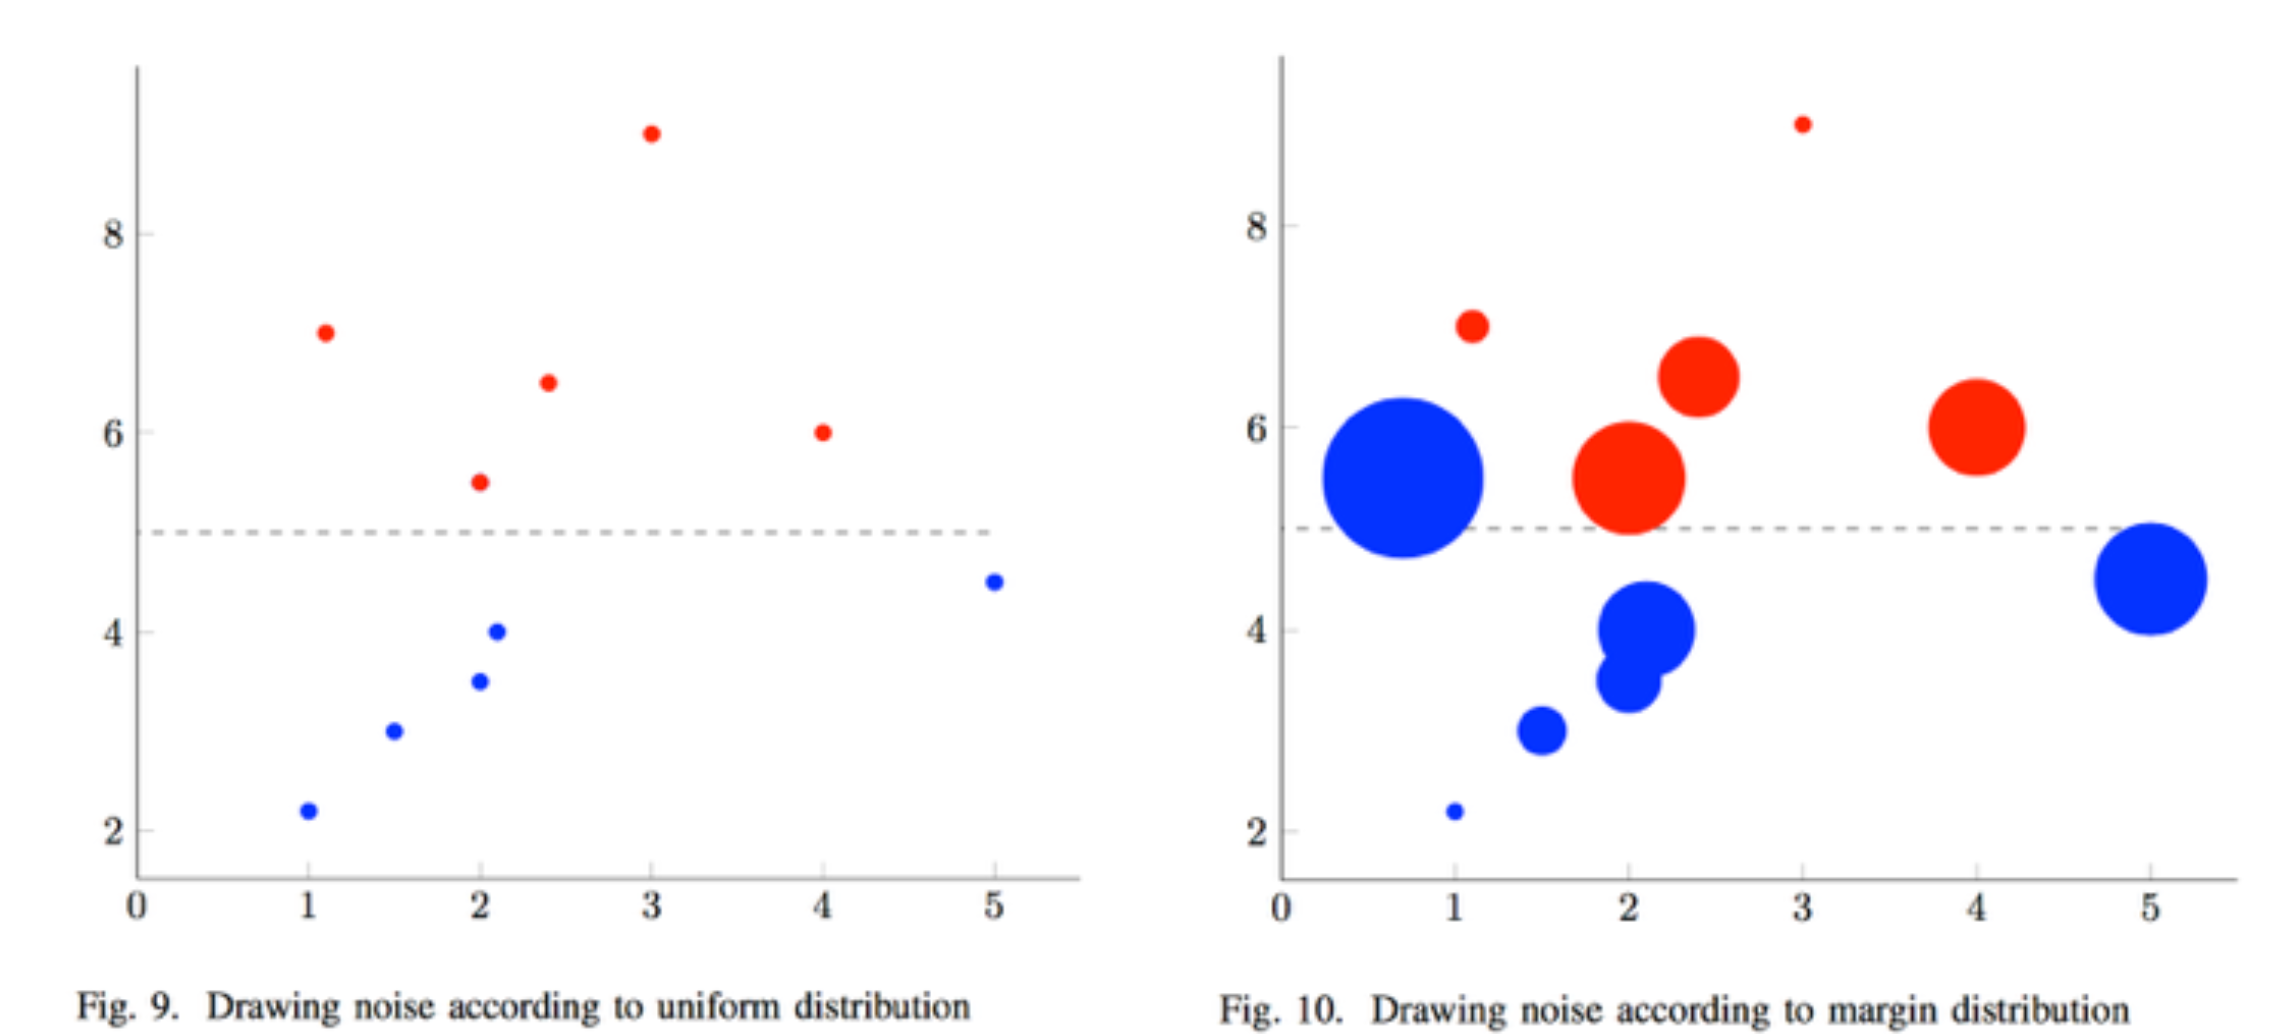
\includegraphics[width=3 in]{figures/Capture.PNG}
\end{figure}
\end{frame}
\section{Results}

\begin{frame}{Experiment Method}
\begin{itemize}
\item
When empirical error is less than $0.05$ at round $t$.
Draw noise points according to $D_{t+1}$.
\item
Test on noise level of 5\%, 10\% and 20\%.
\item
Boosting stumps as base classifier (Threshold function).
\item
Dataset : 80\% Training, 20\% Test
\end{itemize}
\end{frame}

\begin{frame}{AdaBoost Experiment Result}
\begin{figure}%

\subfigure[Adaboost on Ionosphere.]{

\resizebox{0.35\textwidth}{!}{
\begin{tikzpicture}[x=1 in]
\begin{axis}[
	xlabel = Rounds,
	ylabel = Error Rate,
	legend pos= north east
]
\addplot[color=blue] table[x={round}, y={train}]{table/IonoAdaOriginal.txt};
\addplot[color=red] table[x={round}, y={test}]{table/IonoAdaOriginal.txt};
\addplot[dashed, domain=0:50] {0.12};
\legend{original training error,original test error}
\end{axis}
\end{tikzpicture}
}
}
\subfigure[Adaboost 5\% noise.]{
\resizebox{0.35\textwidth}{!}{
\begin{tikzpicture}
\begin{axis}[
	xlabel = Rounds,
	ylabel = Error Rate,
	legend pos= north east
]

\addplot[color=blue] table[x={round}, y={trainmean}]{table/iono_avg_noise_005.txt};
\addplot[color=red] table[x={round}, y={testmean}]{table/iono_avg_noise_005.txt};
\addplot[dashed, domain=0:50] {0.12};
\legend{training error,test error}
\end{axis}
\end{tikzpicture}
}
}\\
\subfigure[Adaboost 10\% noise]{
%\caption{Adaboost running  on Ionosphere.}
\resizebox{0.35\textwidth}{!}{
\begin{tikzpicture}[x=1 in]
\begin{axis}[
	xlabel = Rounds,
	ylabel = Error Rate,
	legend pos= north east
]
\addplot[color=blue] table[x={round}, y={trainmean}]{table/iono_avg_noise_01.txt};
\addplot[color=red] table[x={round}, y={testmean}]{table/iono_avg_noise_01.txt};
\addplot[dashed, domain=0:50] {0.12};
\legend{training error,test error}
\end{axis}
\end{tikzpicture}
}
}
\subfigure[Adaboost 20\% noise.]{
\resizebox{0.35\textwidth}{!}{
\begin{tikzpicture}
\begin{axis}[
	xlabel = Rounds,
	ylabel = Error Rate,
	legend pos= north east
]

\addplot[color=blue] table[x={round}, y={trainmean}]{table/iono_avg_noise_02.txt};
\addplot[color=red] table[x={round}, y={testmean}]{table/iono_avg_noise_02.txt};
\addplot[dashed, domain=0:50] {0.12};
\legend{training error,test error}
\end{axis}
\end{tikzpicture}
}
}
\end{figure}
\end{frame}
\begin{frame}{DeepBoost Experiment Result}
\begin{figure}%

\subfigure[Deeoboost on Ionosphere.]{

\resizebox{0.35\textwidth}{!}{
\begin{tikzpicture}[x=1 in]
\begin{axis}[
	xlabel = Rounds,
	ylabel = Error Rate,
	legend pos= north east
]
\addplot[color=blue] table[x={round}, y={train}]{table/IonoDeepOriginal.txt};
\addplot[color=red] table[x={round}, y={test}]{table/IonoDeepOriginal.txt};
\addplot[dashed, domain=0:50] {0.12};
\legend{original training error,original test error}
\end{axis}
\end{tikzpicture}
}
}
\subfigure[Deepboost 5\% noise.]{
\resizebox{0.35\textwidth}{!}{
\begin{tikzpicture}
\begin{axis}[
	xlabel = Rounds,
	ylabel = Error Rate,
	legend pos= north east
]

\addplot[color=blue] table[x={round}, y={train}]{table/ionodeepn5.txt};
\addplot[color=red] table[x={round}, y={test}]{table/ionodeepn5.txt};
\addplot[dashed, domain=0:50] {0.12};
\legend{training error,test error}
\end{axis}
\end{tikzpicture}
}
}\\
\subfigure[Deepboost 10\% noise]{
%\caption{Adaboost running  on Ionosphere.}
\resizebox{0.35\textwidth}{!}{
\begin{tikzpicture}[x=1 in]
\begin{axis}[
	xlabel = Rounds,
	ylabel = Error Rate,
	legend pos= north east
]
\addplot[color=blue] table[x={round}, y={train}]{table/ionodeepn10.txt};
\addplot[color=red] table[x={round}, y={test}]{table/ionodeepn10.txt};
\addplot[dashed, domain=0:50] {0.12};
\legend{training error,test error}
\end{axis}
\end{tikzpicture}
}
}
\subfigure[Deepboost 20\% noise.]{
\resizebox{0.35\textwidth}{!}{
\begin{tikzpicture}
\begin{axis}[
	xlabel = Rounds,
	ylabel = Error Rate,
	legend pos= north east
]

\addplot[color=blue] table[x={round}, y={train}]{table/ionodeepn20.txt};
\addplot[color=red] table[x={round}, y={test}]{table/ionodeepn20.txt};
\addplot[dashed, domain=0:50] {0.12};
\legend{training error,test error}
\end{axis}
\end{tikzpicture}
}
}
\end{figure}
\end{frame}
\section{}
\begin{frame}
\Huge Thank you!
\end{frame}

\end{document}





















